\documentclass[handout]{ximera}
%\usepackage{todonotes}

\newcommand{\todo}{}

\usepackage{esint} % for \oiint
\graphicspath{
{./}
{functionsOfSeveralVariables/}
{normalVectors/}
{lagrangeMultipliers/}
{vectorFields/}
{greensTheorem/}
{shapeOfThingsToCome/}
}


\usepackage{tkz-euclide}
\tikzset{>=stealth} %% cool arrow head
\tikzset{shorten <>/.style={ shorten >=#1, shorten <=#1 } } %% allows shorter vectors

\usetikzlibrary{backgrounds} %% for boxes around graphs
\usetikzlibrary{shapes,positioning}  %% Clouds and stars
\usetikzlibrary{matrix} %% for matrix
\usepgfplotslibrary{polar} %% for polar plots
\usetkzobj{all}
\usepackage[makeroom]{cancel} %% for strike outs
%\usepackage{mathtools} %% for pretty underbrace % Breaks Ximera
\usepackage{multicol}
\usepackage{pgffor} %% required for integral for loops


%% http://tex.stackexchange.com/questions/66490/drawing-a-tikz-arc-specifying-the-center
%% Draws beach ball
\tikzset{pics/carc/.style args={#1:#2:#3}{code={\draw[pic actions] (#1:#3) arc(#1:#2:#3);}}}



\usepackage{array}
\setlength{\extrarowheight}{+.1cm}   
\newdimen\digitwidth
\settowidth\digitwidth{9}
\def\divrule#1#2{
\noalign{\moveright#1\digitwidth
\vbox{\hrule width#2\digitwidth}}}





\newcommand{\RR}{\mathbb R}
\newcommand{\R}{\mathbb R}
\newcommand{\N}{\mathbb N}
\newcommand{\Z}{\mathbb Z}

%\newcommand{\sage}{\textsf{SageMath}}


%\renewcommand{\d}{\,d\!}
\renewcommand{\d}{\mathop{}\!d}
\newcommand{\dd}[2][]{\frac{\d #1}{\d #2}}
\newcommand{\pp}[2][]{\frac{\partial #1}{\partial #2}}
\renewcommand{\l}{\ell}
\newcommand{\ddx}{\frac{d}{\d x}}

\newcommand{\zeroOverZero}{\ensuremath{\boldsymbol{\tfrac{0}{0}}}}
\newcommand{\inftyOverInfty}{\ensuremath{\boldsymbol{\tfrac{\infty}{\infty}}}}
\newcommand{\zeroOverInfty}{\ensuremath{\boldsymbol{\tfrac{0}{\infty}}}}
\newcommand{\zeroTimesInfty}{\ensuremath{\small\boldsymbol{0\cdot \infty}}}
\newcommand{\inftyMinusInfty}{\ensuremath{\small\boldsymbol{\infty - \infty}}}
\newcommand{\oneToInfty}{\ensuremath{\boldsymbol{1^\infty}}}
\newcommand{\zeroToZero}{\ensuremath{\boldsymbol{0^0}}}
\newcommand{\inftyToZero}{\ensuremath{\boldsymbol{\infty^0}}}



\newcommand{\numOverZero}{\ensuremath{\boldsymbol{\tfrac{\#}{0}}}}
\newcommand{\dfn}{\textbf}
%\newcommand{\unit}{\,\mathrm}
\newcommand{\unit}{\mathop{}\!\mathrm}
\newcommand{\eval}[1]{\bigg[ #1 \bigg]}
\newcommand{\seq}[1]{\left( #1 \right)}
\renewcommand{\epsilon}{\varepsilon}
\renewcommand{\phi}{\varphi}


\renewcommand{\iff}{\Leftrightarrow}

\DeclareMathOperator{\arccot}{arccot}
\DeclareMathOperator{\arcsec}{arcsec}
\DeclareMathOperator{\arccsc}{arccsc}
\DeclareMathOperator{\si}{Si}
\DeclareMathOperator{\proj}{\vec{proj}}
\DeclareMathOperator{\scal}{scal}
\DeclareMathOperator{\sign}{sign}


%% \newcommand{\tightoverset}[2]{% for arrow vec
%%   \mathop{#2}\limits^{\vbox to -.5ex{\kern-0.75ex\hbox{$#1$}\vss}}}
\newcommand{\arrowvec}{\overrightarrow}
%\renewcommand{\vec}[1]{\arrowvec{\mathbf{#1}}}
\renewcommand{\vec}{\mathbf}
\newcommand{\veci}{{\boldsymbol{\hat{\imath}}}}
\newcommand{\vecj}{{\boldsymbol{\hat{\jmath}}}}
\newcommand{\veck}{{\boldsymbol{\hat{k}}}}
\newcommand{\vecl}{\boldsymbol{\l}}
\newcommand{\uvec}[1]{\mathbf{\hat{#1}}}
\newcommand{\utan}{\mathbf{\hat{t}}}
\newcommand{\unormal}{\mathbf{\hat{n}}}
\newcommand{\ubinormal}{\mathbf{\hat{b}}}

\newcommand{\dotp}{\bullet}
\newcommand{\cross}{\boldsymbol\times}
\newcommand{\grad}{\boldsymbol\nabla}
\newcommand{\divergence}{\grad\dotp}
\newcommand{\curl}{\grad\cross}
%\DeclareMathOperator{\divergence}{divergence}
%\DeclareMathOperator{\curl}[1]{\grad\cross #1}
\newcommand{\lto}{\mathop{\longrightarrow\,}\limits}

\renewcommand{\bar}{\overline}

\colorlet{textColor}{black} 
\colorlet{background}{white}
\colorlet{penColor}{blue!50!black} % Color of a curve in a plot
\colorlet{penColor2}{red!50!black}% Color of a curve in a plot
\colorlet{penColor3}{red!50!blue} % Color of a curve in a plot
\colorlet{penColor4}{green!50!black} % Color of a curve in a plot
\colorlet{penColor5}{orange!80!black} % Color of a curve in a plot
\colorlet{penColor6}{yellow!70!black} % Color of a curve in a plot
\colorlet{fill1}{penColor!20} % Color of fill in a plot
\colorlet{fill2}{penColor2!20} % Color of fill in a plot
\colorlet{fillp}{fill1} % Color of positive area
\colorlet{filln}{penColor2!20} % Color of negative area
\colorlet{fill3}{penColor3!20} % Fill
\colorlet{fill4}{penColor4!20} % Fill
\colorlet{fill5}{penColor5!20} % Fill
\colorlet{gridColor}{gray!50} % Color of grid in a plot

\newcommand{\surfaceColor}{violet}
\newcommand{\surfaceColorTwo}{redyellow}
\newcommand{\sliceColor}{greenyellow}




\pgfmathdeclarefunction{gauss}{2}{% gives gaussian
  \pgfmathparse{1/(#2*sqrt(2*pi))*exp(-((x-#1)^2)/(2*#2^2))}%
}


%%%%%%%%%%%%%
%% Vectors
%%%%%%%%%%%%%

%% Simple horiz vectors
\renewcommand{\vector}[1]{\left\langle #1\right\rangle}


%% %% Complex Horiz Vectors with angle brackets
%% \makeatletter
%% \renewcommand{\vector}[2][ , ]{\left\langle%
%%   \def\nextitem{\def\nextitem{#1}}%
%%   \@for \el:=#2\do{\nextitem\el}\right\rangle%
%% }
%% \makeatother

%% %% Vertical Vectors
%% \def\vector#1{\begin{bmatrix}\vecListA#1,,\end{bmatrix}}
%% \def\vecListA#1,{\if,#1,\else #1\cr \expandafter \vecListA \fi}

%%%%%%%%%%%%%
%% End of vectors
%%%%%%%%%%%%%

%\newcommand{\fullwidth}{}
%\newcommand{\normalwidth}{}



%% makes a snazzy t-chart for evaluating functions
%\newenvironment{tchart}{\rowcolors{2}{}{background!90!textColor}\array}{\endarray}

%%This is to help with formatting on future title pages.
\newenvironment{sectionOutcomes}{}{} 



%% Flowchart stuff
%\tikzstyle{startstop} = [rectangle, rounded corners, minimum width=3cm, minimum height=1cm,text centered, draw=black]
%\tikzstyle{question} = [rectangle, minimum width=3cm, minimum height=1cm, text centered, draw=black]
%\tikzstyle{decision} = [trapezium, trapezium left angle=70, trapezium right angle=110, minimum width=3cm, minimum height=1cm, text centered, draw=black]
%\tikzstyle{question} = [rectangle, rounded corners, minimum width=3cm, minimum height=1cm,text centered, draw=black]
%\tikzstyle{process} = [rectangle, minimum width=3cm, minimum height=1cm, text centered, draw=black]
%\tikzstyle{decision} = [trapezium, trapezium left angle=70, trapezium right angle=110, minimum width=3cm, minimum height=1cm, text centered, draw=black]
\author{Mary E. Pilgrim, and implemented in Ximera by Ben Sencindiver}
   

\title{Spring 2017 Exam 2}

\begin{document}
\begin{abstract}
  Here you can work on a practice exam 2. This exam was administered in Spring 2017.
\end{abstract}
\maketitle


\begin{center}
\Large{Math 160 Calculus for Physical Scientists I \\ Exam 2 - Version 1 \\ March 9, 2017, 5:00-6:50 pm}
\end{center}


%%MC%%
\begin{problem}
If the radius of a circle increases from $r=A$ to $r=B$, then the average rate of change of the area of the circle is

\begin{multipleChoice}
	\choice{$\pi(B^2-A^2)$}
	\choice{$\pi(B-A)$}
	\choice{$\displaystyle\pi\left(B^2+A^2\right)$}
	\choice[correct]{$\displaystyle\pi\left(B+A\right)$}
	\choice{None of the above}
\end{multipleChoice}
\end{problem}


%%%%% Here!!!!1

\begin{problem}
We know that $f(2)=4$ and $f'(2)=3$, then the value of $\displaystyle\frac{d}{dx}\left(\frac{3x^2}{f(x)}\right)\bigg|_{x=2}$

%%% Add Answer here.
\begin{multipleChoice}
	\choice{$\displaystyle\frac{21}{4}$}
	\choice{$\displaystyle\frac{4}{3}$}
	\choice[correct]{$\displaystyle\frac{3}{4}$}
	\choice{4}
	\choice{None of the above.}\\
\end{multipleChoice}
\end{problem}


%%%% Add the solution %%%%
\begin{problem}
If $h'(t)$ is continuous on $(-\infty,\infty)$, then 
\begin{multipleChoice}
	\choice{$\displaystyle\lim_{t\rightarrow100}h(t)=h'(100)$.}
    \choice[correct]{$\displaystyle \lim_{t\rightarrow100} h(t)= h(100)$.}
	\choice{$\displaystyle\lim_{t\rightarrow100}h(t)$ \hspace{0.2in} may not exist.}
	\choice{$\displaystyle\lim_{h\rightarrow0}\frac{h(100+h)-h(100)}{h}$ may not exist.}
	\choice{None of the above.}
\end{multipleChoice}
\end{problem}

%%VELOCITY - MC%%
\begin{problem}
The function $f(t)$ represents the distance of a vehicle moving along a straight road from its starting point at time $t$. 

Below are three graphs of the derivative, $f'(t)$, of the distance function. Which graph best matches each of the following vehicle scenarios?

Graph 1: 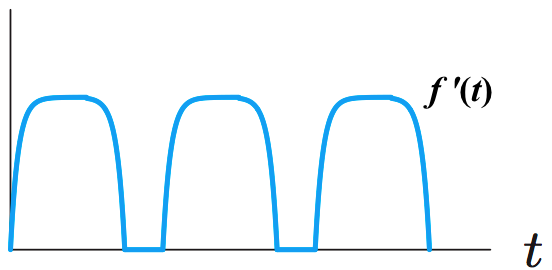
\includegraphics[scale=0.25]{Bus-A.png}

Graph 2: 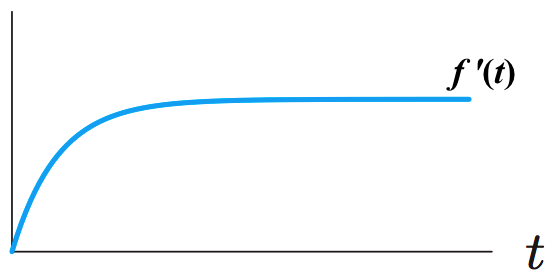
\includegraphics[scale=0.25]{Car-A.png}

Graph 3: 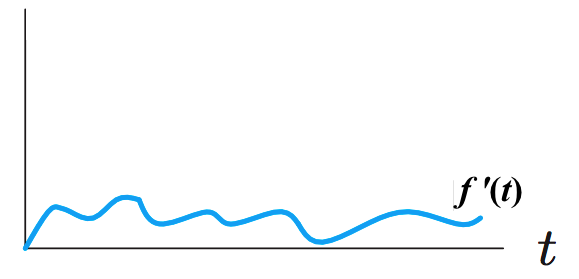
\includegraphics[scale=0.25]{Car-traffic-A.png}


\begin{question}
\underline{Scenario 1}: A car in heavy traffic conditions.
\begin{multipleChoice}
    \choice{Graph 1}
    \choice{Graph 2}
    \choice[correct]{Graph 3}
\end{multipleChoice}
\end{question}

\begin{question}
\underline{Scenario 2}: A bus on a popular route, with no traffic.
\begin{multipleChoice}
    \choice[correct]{Graph 1}
    \choice{Graph 2}
    \choice{Graph 3}
\end{multipleChoice}
\end{question}

\begin{question}
\underline{Scenario 3}: A car with no traffic and all green lights.
\begin{multipleChoice}
    \choice{Graph 1}
    \choice[correct]{Graph 2}
    \choice{Graph 3}
\end{multipleChoice}
\end{question}

\end{problem}


%%CURVE SKETCH%%
\begin{problem}
Below is the graph of the function, $f(x)$. 

\bigskip

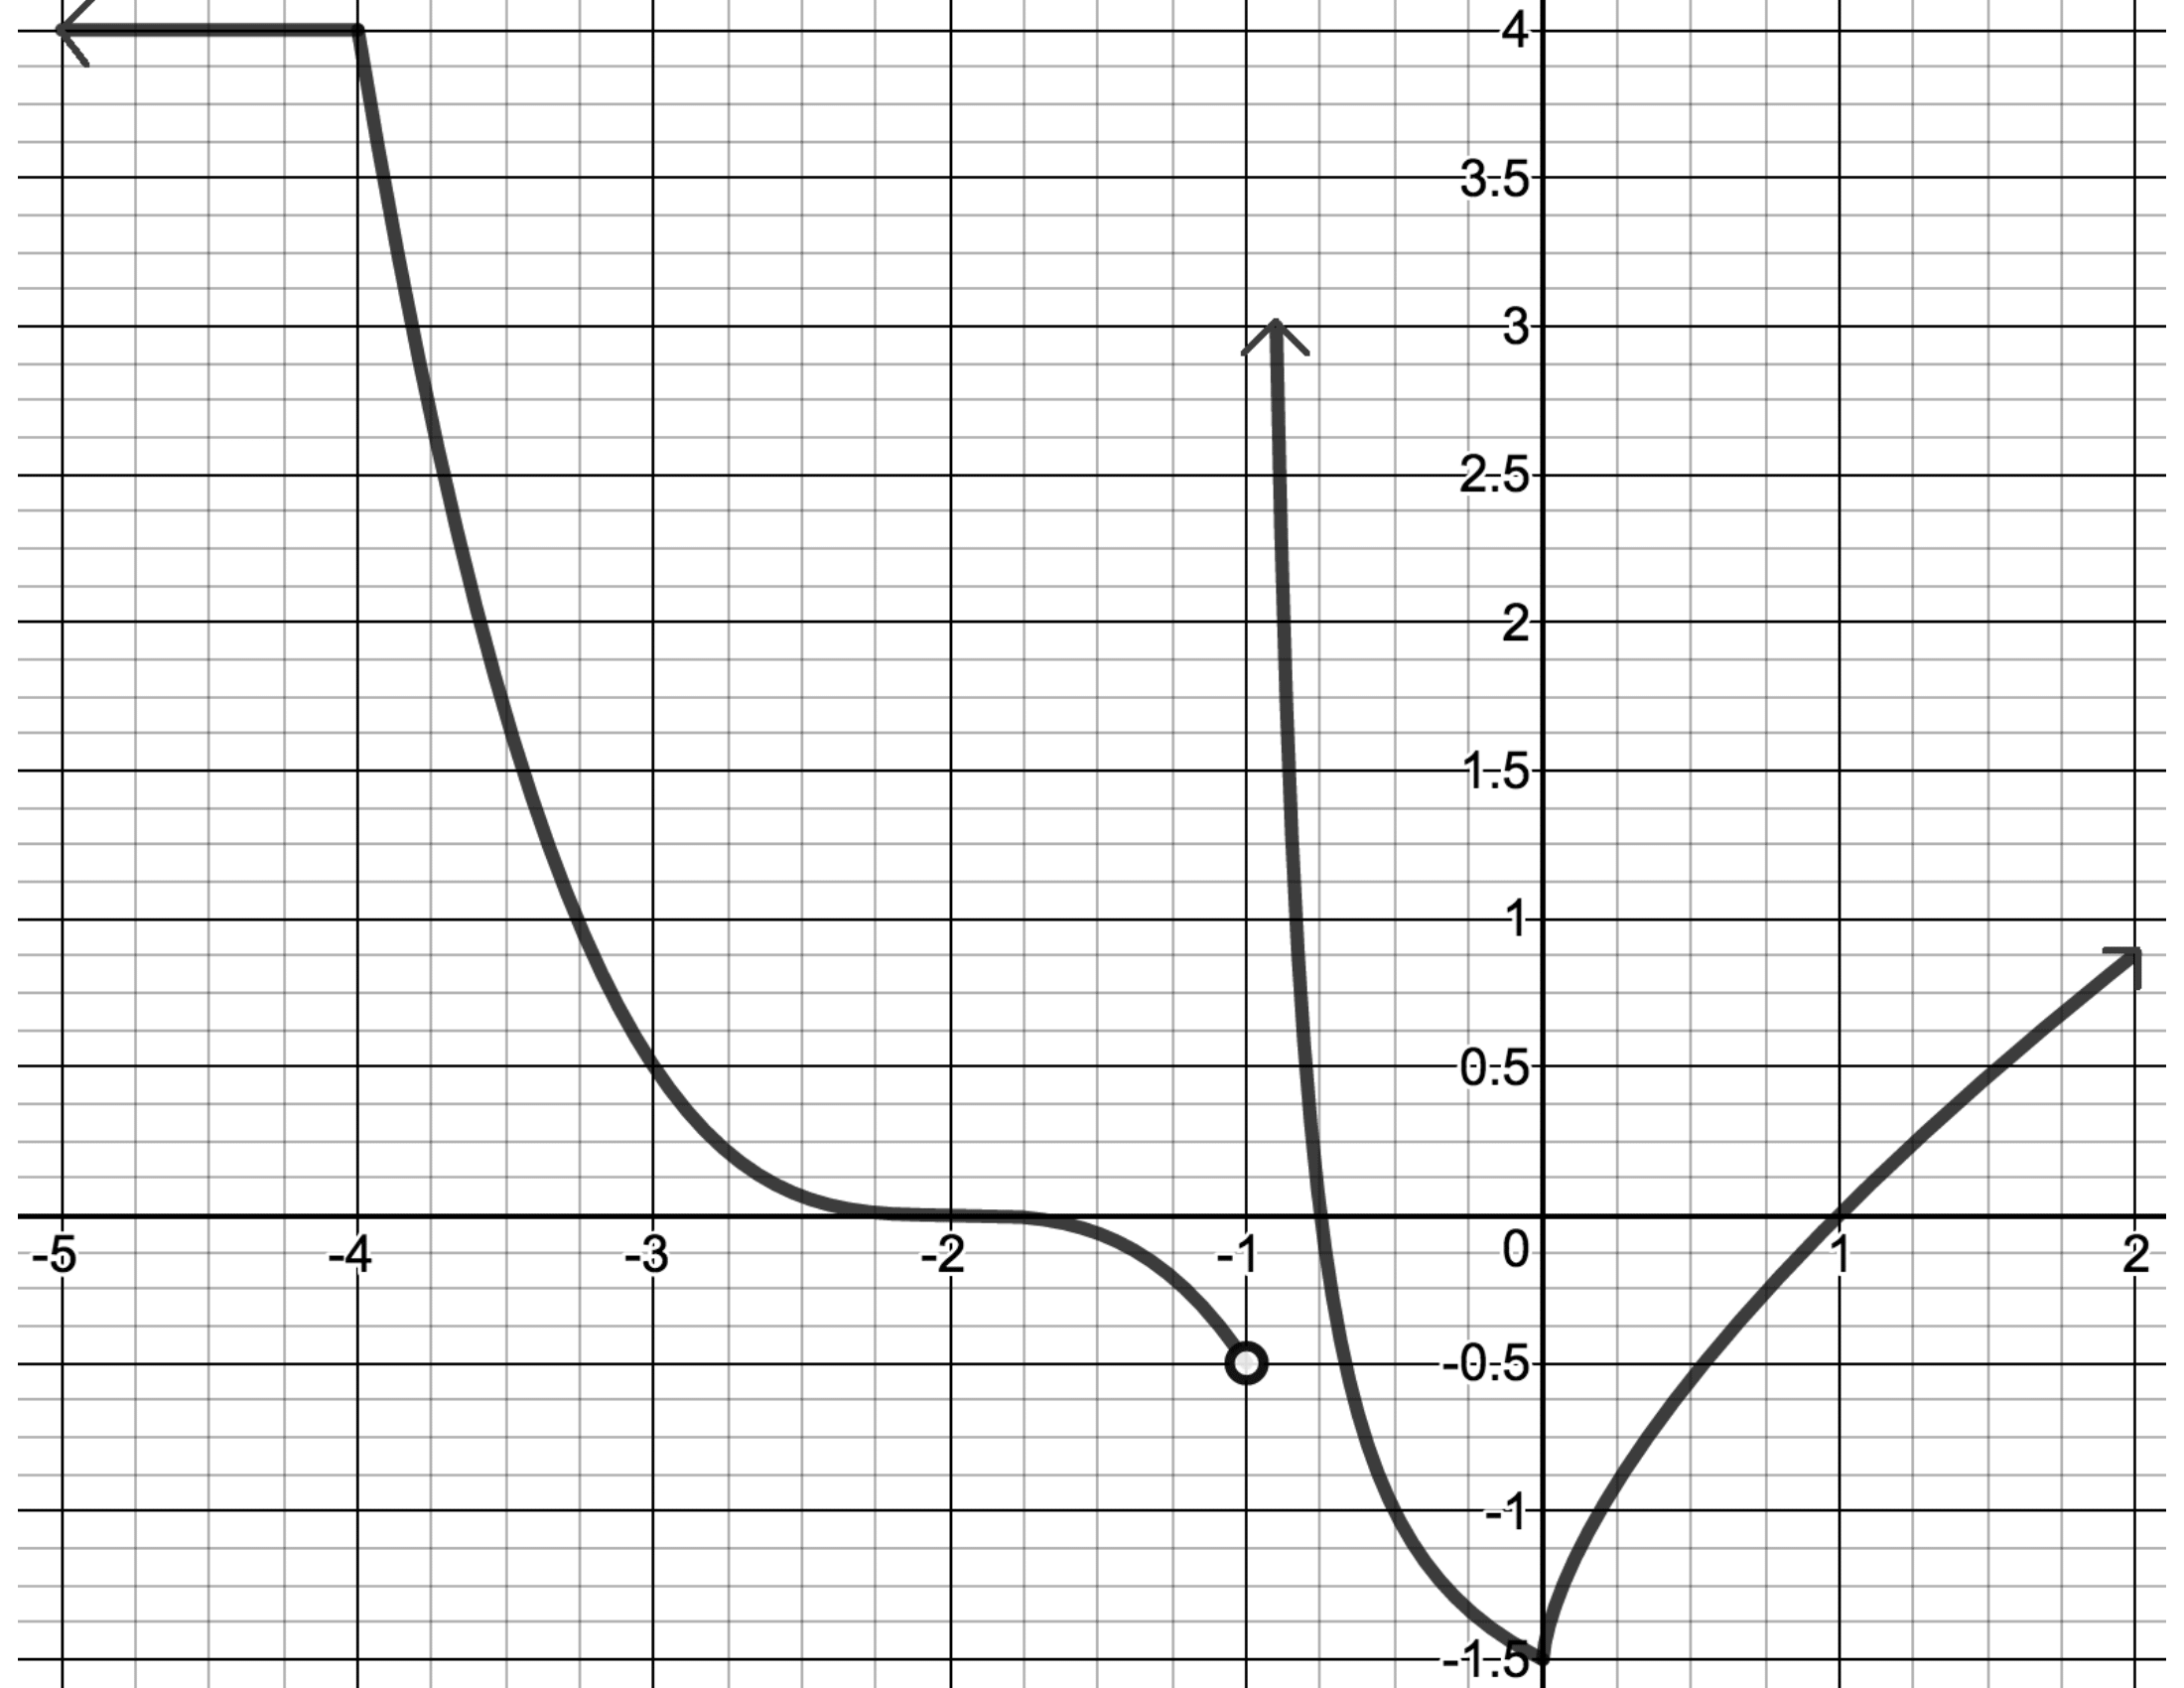
\includegraphics[scale=0.1]{CurveSketch-Ex2sp17.png}

Of all the properties listed below, choose all properties that are reflected in the graph of $f(x)$.

\begin{multicols}
\begin{selectAll}
	\choice{$f(x)$ is not continuous at $x=-4$}
	\choice[correct]{$f(x)$ is not continuous at $x=-1$}
	\choice{$f(x)$ is not continuous at $x=0$}
	\choice[correct]{$f(x)$ is not differentiable at $x=-4$}
	\choice[correct]{$f(x)$ is not differentiable at $x=-1$}
	\choice[correct]{$f(x)$ is not differentiable at $x=0$}
	\choice[correct]{$f'(x)=0$ at $x=-2$}
	\choice{$f'(x)=0$ at $x=0$}
	\choice[correct]{$f'(x)<0$ for $-4<x<-2$}
	\choice[correct]{$f'(x)<0$ for $-2<x<-1$}
	\choice[correct]{$f'(x)<0$ for $-1<x<0$}
	\choice{$f'(x)<0$ for $x>0$}
	\choice{$f'(x)>0$ for $-4<x<-2$}
	\choice{$f'(x)>0$ for $-2<x<-1$}
	\choice{$f'(x)>0$ for $-1<x<0$}
	\choice[correct]{$f'(x)>0$ for $x>0$}
	\choice{$y=4$ is an absolute maximum}
	\choice{$y=3$ is an absolute maximum}
	\choice{$y=-0.5$ is an absolute minimum}
	\choice[correct]{$y=-1.5$ is an absolute minimum}
\end{selectAll}
\end{problems}
\end{problem}

%%DERIVATIVES%%
\begin{problem}
Use $g(t)=\tan(f(t))$ to answer the following. When referring to $f'(t)$, use $d(t)$.

	\begin{question}
	Find the derivative of $g(t)$.
	
    \[
    \answer[given]{(\sec(f(t)))^2 * d(t)}
    \]
    \end{question}
    
	
	\begin{question}
    Using your result from part (a) and the information provided in the table below, find the value of $g'(\pi)$. Circle the correct answer.

\[
    \begin{array}{c||c|c}
	\, & f(t) & f'(t)\\
     \hline\hline
	\, & \, & \, \\
	t=0 & 2 & -\frac{1}{2}\\
	\, & \, & \, \\
	\hline
	\, & \, & \, \\
	t=\pi & \frac{\pi}{3} & \pi\\
    \end{array}
\]
	
    \begin{multipleChoice}
	    \choice[correct]{$g'(\pi)=4\pi$}
	    \choice{$g'(\pi)=4$}
	    \choice{$g'(\pi)=\pi$}
	    \choice{$g'(\pi)=0$}
	    \choice{$g'(\pi)=1$}
    \end{multipleChoice}
    \end{question}
\end{problem}



\begin{problem}
Suppose that $f(t)=3t$, then $g(t)=\tan(3t)$.\\

What is $g''(t)$? Circle the correct answer.

\begin{multipleChoice}
	\choice{$3\sec^2(3t)$}
	\choice[correct]{$18\sec^2(3t)\tan(3t)$}
	\choice{$2\sec^2(3t)\tan(3t)$}
	\choice{$6\sec^2(3t)\tan(3t)$}
	\choice{$2\sec(3t)$}
\end{multipleChoice}
\end{problem}


\begin{problem}
Below is the graph of the implicitly defined function $\displaystyle\sin \left(\pi y\right)+3y^2=3x^3$. 

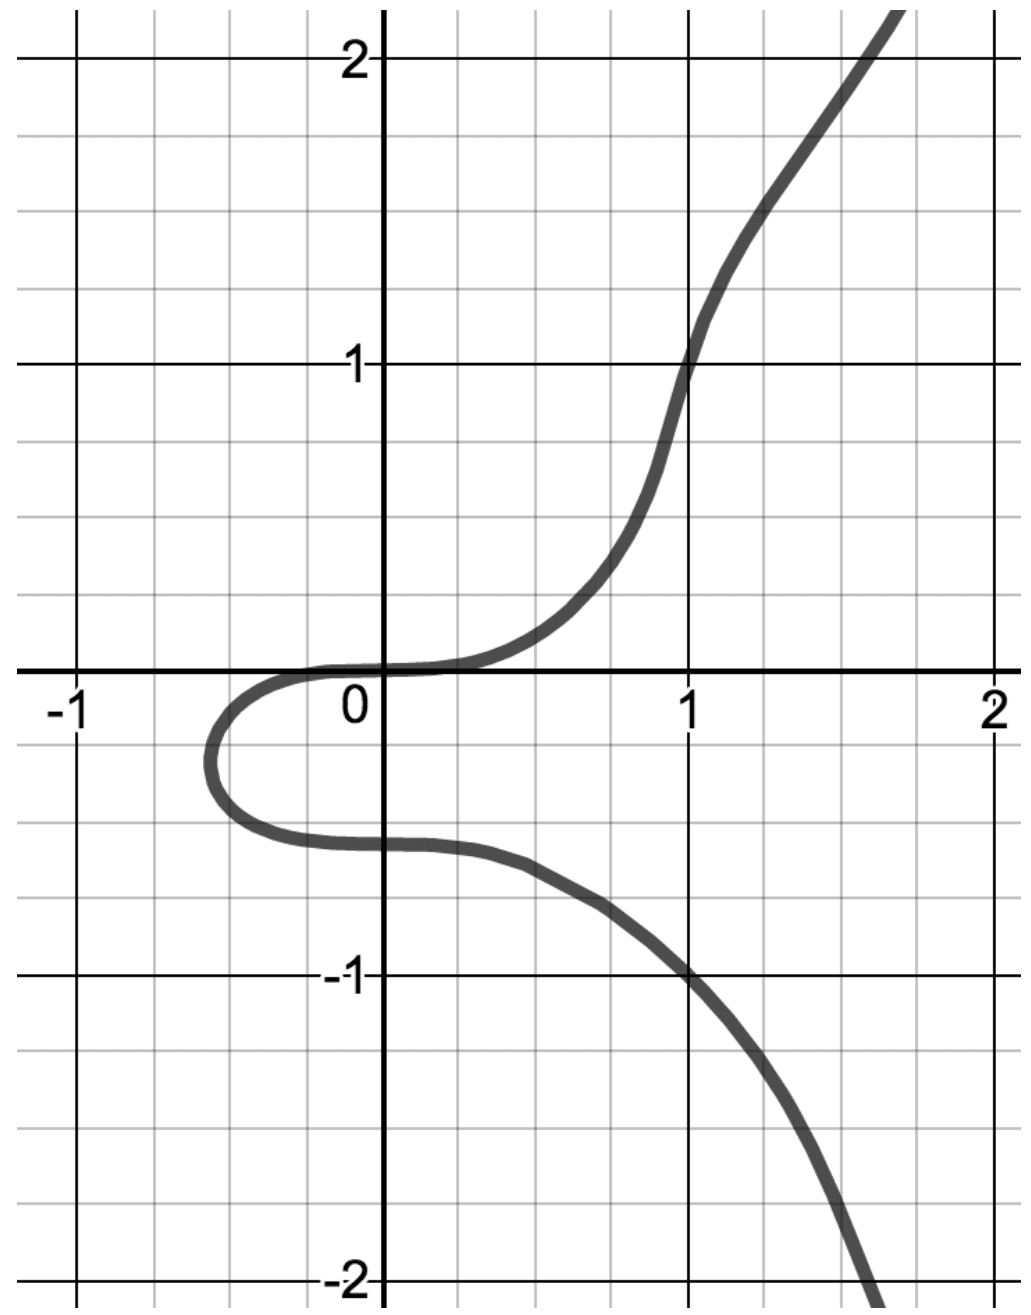
\includegraphics[scale=0.1]{Exam2-ImpDiff2.png}


	\begin{question}
	It can be seen in the picture that the point $(1,-1)$ is on the graph of $\displaystyle\sin \left(\pi y\right)+3y^2=3x^3$. Algebraically verify this fact. (Note that your response cannot be validated as correct or incorrect in this system).\\
    \begin{freeResponse}
    \end{freeResponse}
    \end{question}
    
	
	\begin{question}
    Use calculus to find $\displaystyle\frac{dy}{dx}$.\\
    
    \[
    \displaystyle \dfrac{dy}{dx} = \answer[given]{\dfrac{9x^2}{\pi *\cos(\pi*y) + 6y}}
    \]
    \end{question}
    

	\begin{question}
    Find the slope of the line tangent to $\displaystyle\sin \left(\pi y\right)+3y^2=3x^3$ at the point $(1,-1)$.\\
    
    The slope of the line is $\answer[given]{\dfrac{9}{-1(\pi +6)}}$.
    \end{question}
	
	\begin{question}
    Find the equation of the line tangent to $\displaystyle\sin \left(\pi y\right)+3y^2=3x^3$ at the point $(1,-1)$. \\
    
    In point-slope form, the equation of the line tangent to the curve at $(1,-1)$ is \\
    
    \[
    y - \answer[given]{-1} = \answer[given]{\dfrac{9}{-1(\pi +6)}} ( x - \answer[given]{1}).
    \]
    \end{question}
\end{problem}

%%TRUE FALSE%%
\begin{problem}
Indicate whether each of the following statements is \textbf{True} or \textbf{False}.

If the statement is true, explain how you know it's true.\\



If it is false, give a counterexample \textbf{and} explain why it is a counterexample. (A counterexample is an example of a function for which the ``if'' part of the statement is true, but the ``then'' part is false.) \underline{A graph with an explanation can be used as a counterexample.}\\


\begin{question}
If $f$ is continuous at $x=1$, then $f$ is differentiable at $x=1$
    \begin{multipleChoice}
	    \choice{True}
	    \choice[correct]{False}
    \end{multipleChoice}
\end{question}


\begin{question}
	Given that $f(x)$ is continuous on the interval $(1,3)$, then $f(x)$ attains an absolute maximum on the interval $(1,3)$.\\
    
    \begin{multipleChoice}
	    \choice{True}
	    \choice[correct]{False}
    \end{multipleChoice}
\end{question}


\begin{question}
    Two different functions, $f(x)$ and $g(x)$, cannot have the same derivative functions unless both $f(x)$ and $g(x)$ are linear functions with the same slope.
    \begin{multipleChoice}
	    \choice{True}
	    \choice[correct]{False}
    \end{multipleChoice}
\end{question}

\end{problem}


\begin{problem}
Consider the function $f(x)$ given by

$$f(x) = \begin{cases} \displaystyle -x^3, & x \leq 0 \\ x^3, & x >0 \end{cases}$$

\begin{question}
Use the \textbf{definition of the derivative} of a function at a point (as a limit) to determine whether $f(x)$ is differentiable at $x=0$. Show details of how you made this determination. Evaluate any limits involved algebraically (without using a calculator).

If $f'(0)$ exists, fill in the blank with its value. If not, draw a smiley face in the blank. (Type DNE if the limit doesn't exist.) \\
\[
\displaystyle \lim_{h\to 0^-} \dfrac{f(0+h) - f(0)}{h} = \displaystyle \lim_{h\to 0^-} \answer[given]{\dfrac{-h^3}{h}} = \answer[given]{0}
\]

\[
\displaystyle \lim_{h\to 0^-} \dfrac{f(0+h) - f(0)}{h} = \displaystyle \lim_{h\to 0^+} \answer[given]{\dfrac{h^3}{h}} = \answer[given]{0}
\]

so

\[
f'(0) = \answer[given]{0}
\]
\end{question}

% Not sure how to make this into a question.
\begin{question}
Sketch a graph of $f(x)$ on the grid provided. \\(Note that this question cannot be validated in this system.)

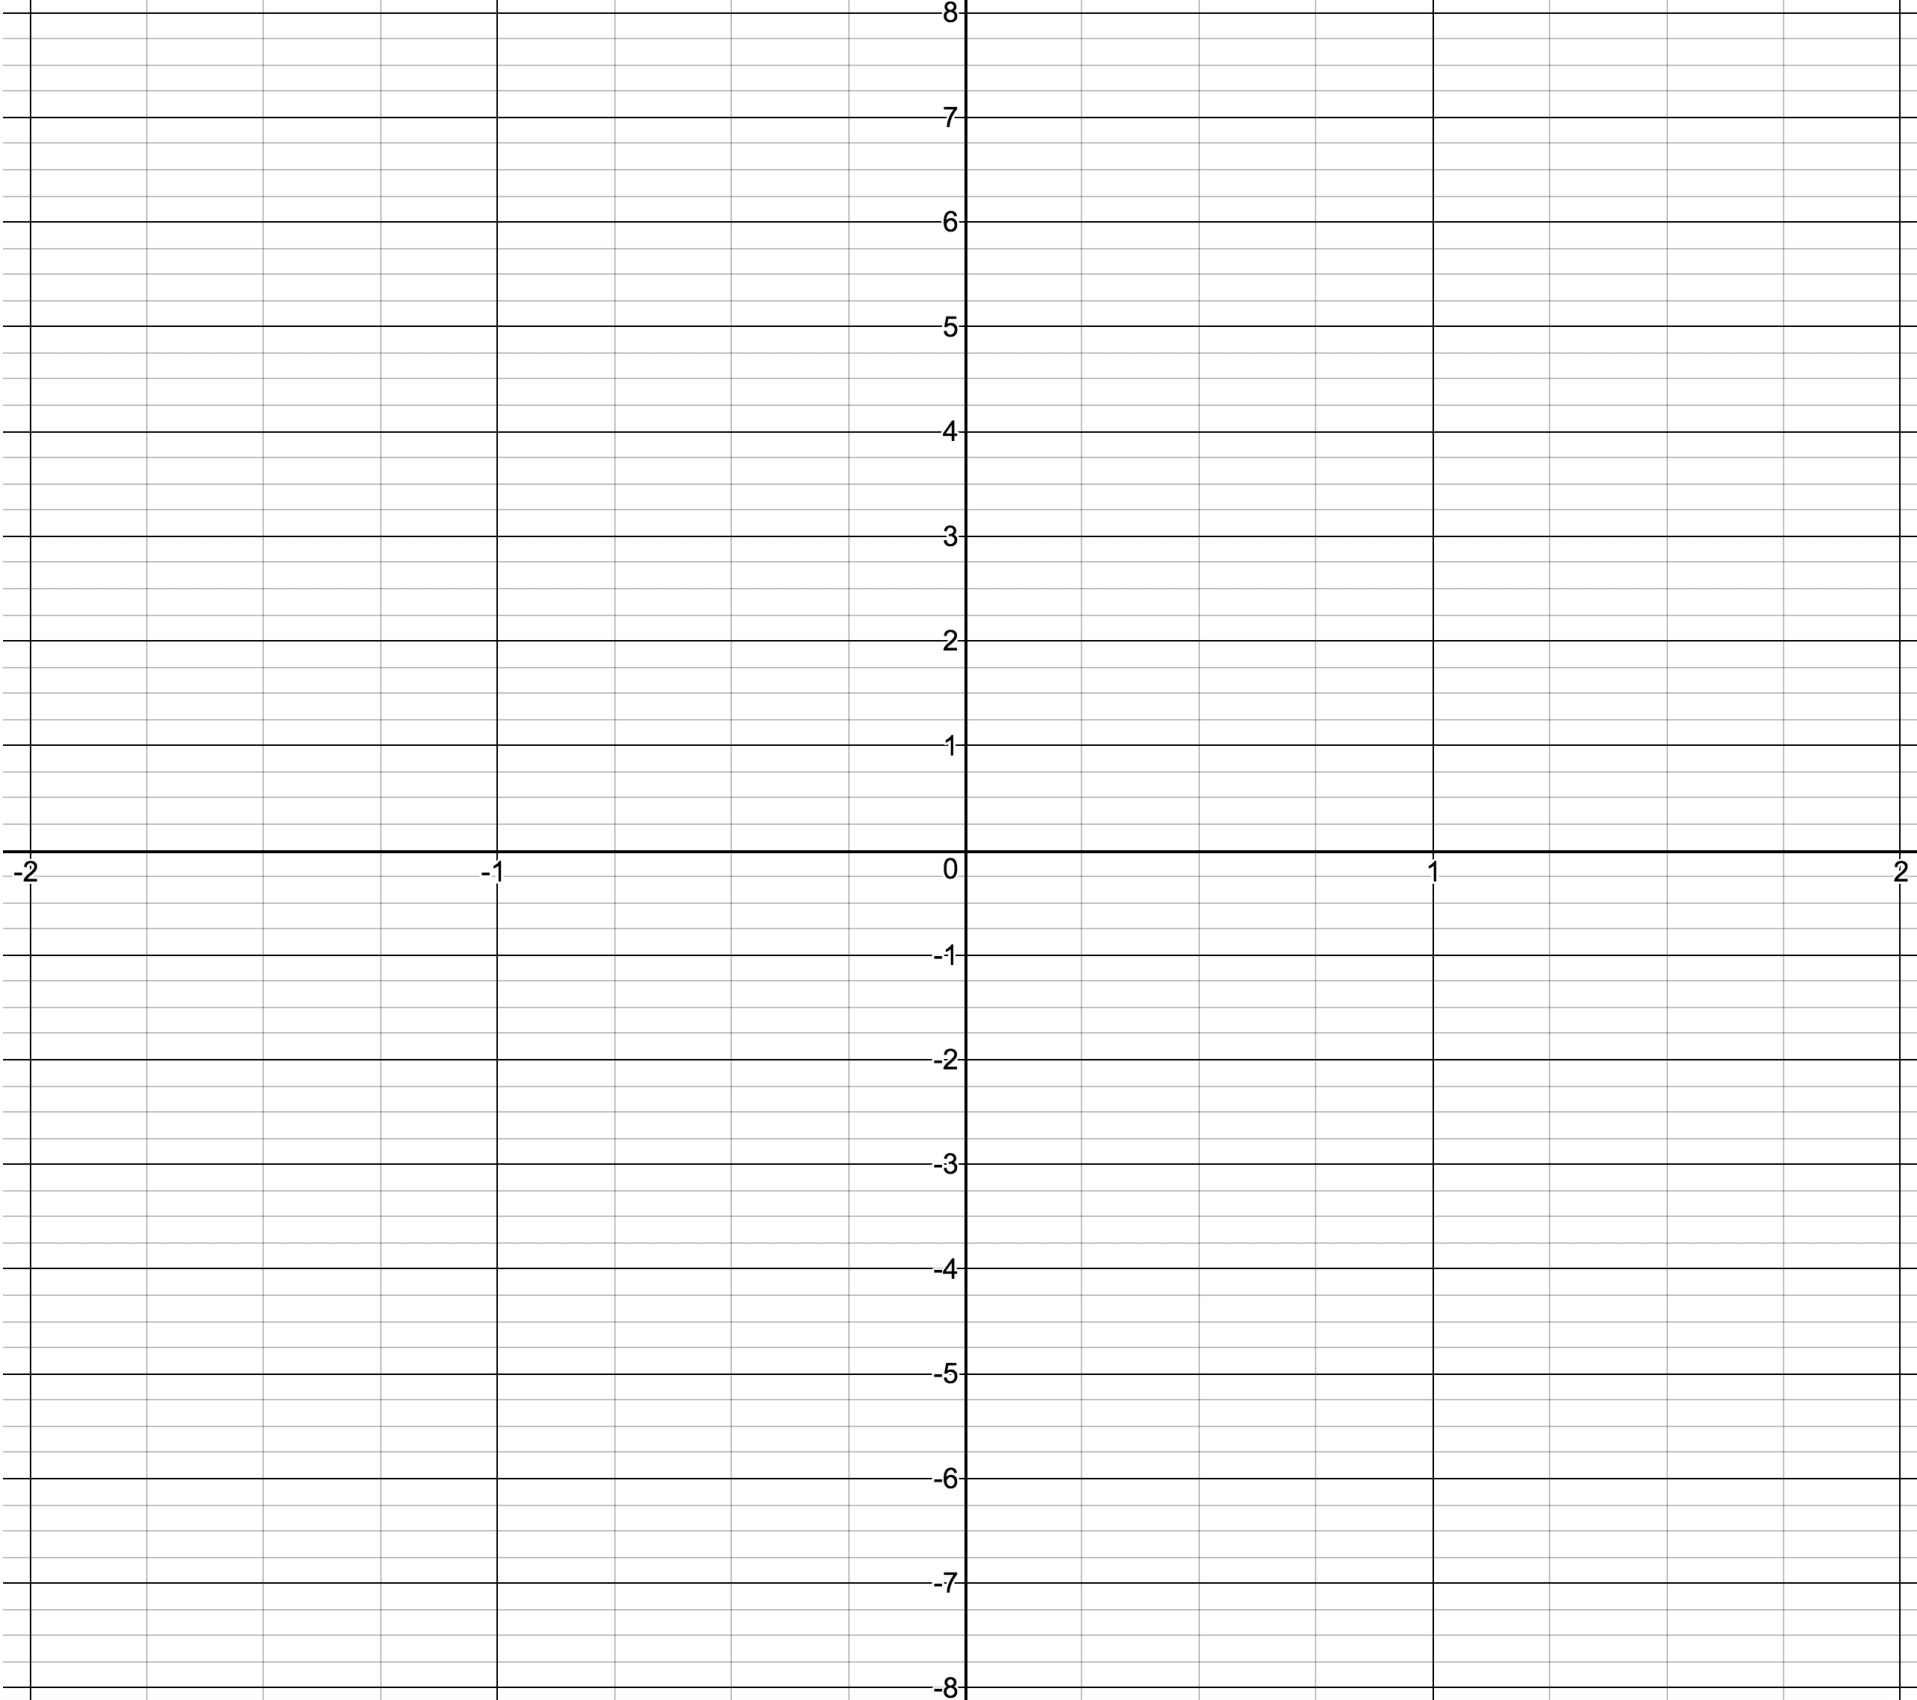
\includegraphics[scale=0.05]{2X8.png}
\end{question}

\begin{question}
Describe how your graph above supports the answer you found in the first question of this problem. \\(Note that this question cannot be validated in this system.)
\begin{freeResponse}
\end{freeResponse}
\end{question}
\end{problem}

\begin{problem}
There are three graphs plotted in the coordinate system below ($f(x)$, $f'(x)$, and $f''(x)$). 


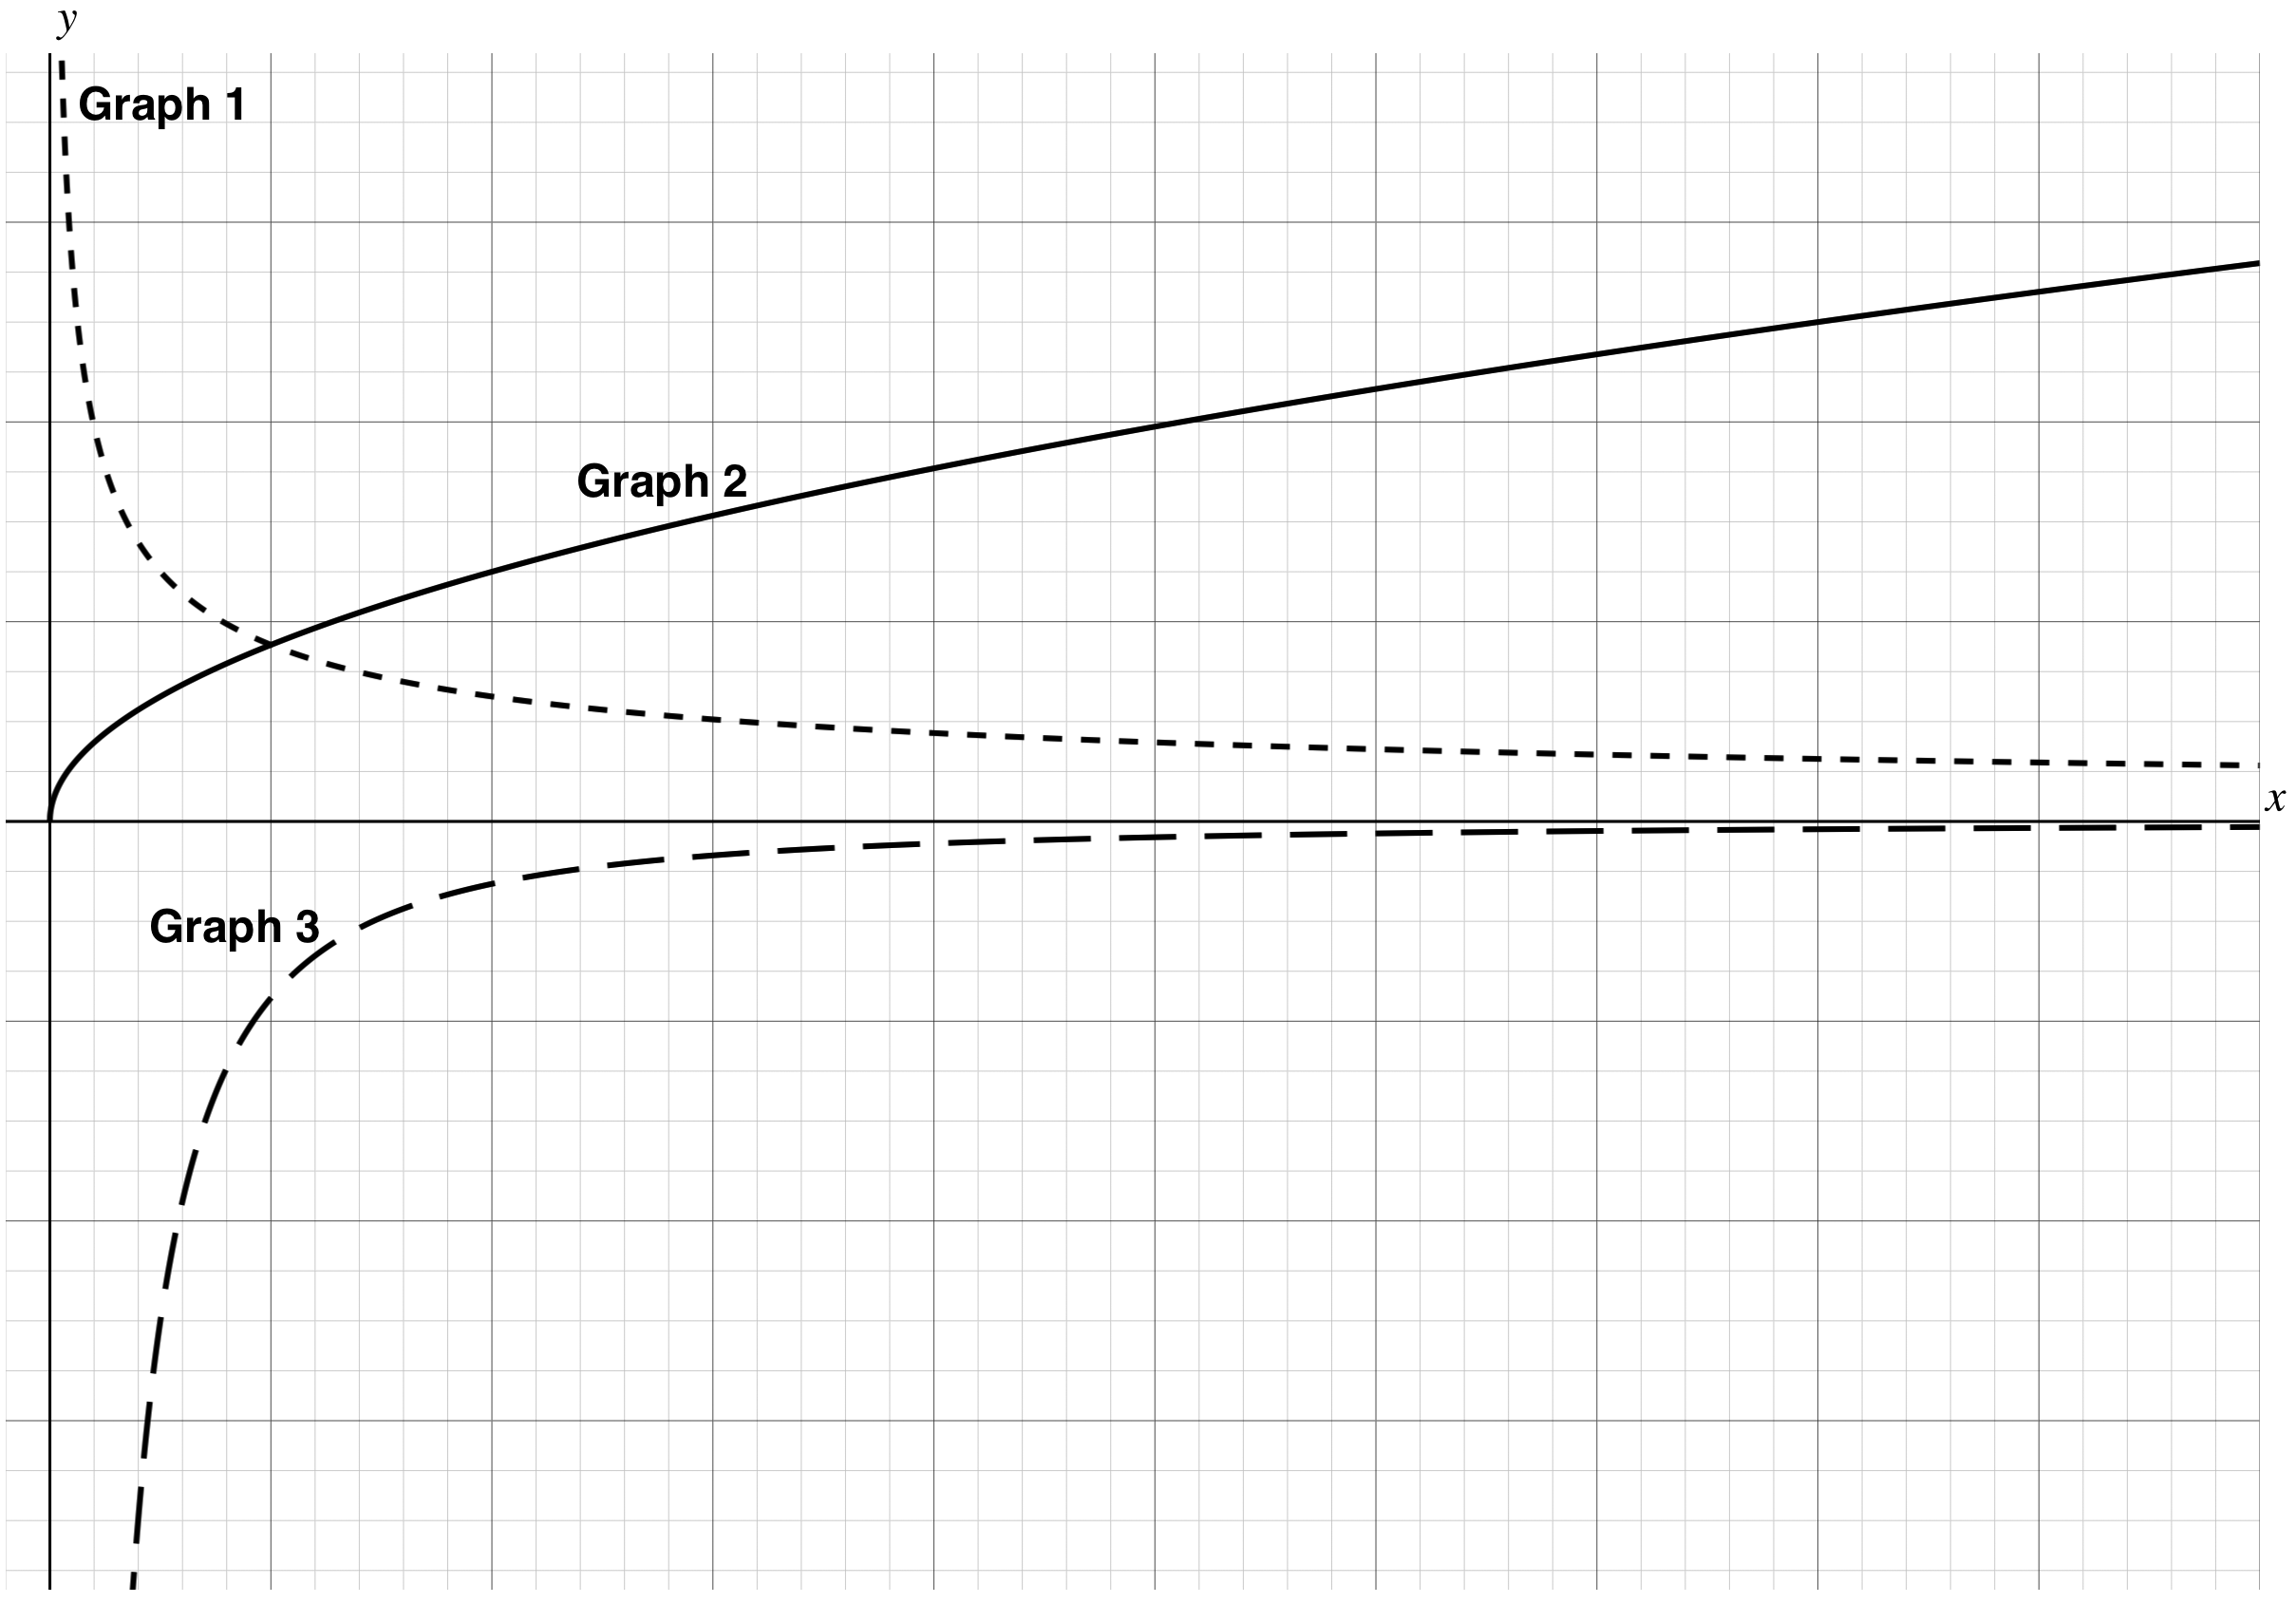
\includegraphics[scale=.01]{SVA-label.png}


Which graph is $f(x)$? Which graph is $f'(x)$? Which graph is $f''(x)$? Give reasons for your answers in sentences. Your explanation should include a discussion of slope with regard to each graph.

\begin{question}
Graph 1 is
\begin{multipleChoice}
    \choice{$f(x)$}
    \choice[correct]{$f'(x)$}
    \choice{$f''(x)$}
\end{multipleChoice}
\end{question}

\begin{question}
Graph 2 is
\begin{multipleChoice}
    \choice[correct]{$f(x)$}
    \choice{$f'(x)$}
    \choice{$f''(x)$}
\end{multipleChoice}
\end{question}

\begin{question}
Graph 3 is
\begin{multipleChoice}
    \choice{$f(x)$}
    \choice{$f'(x)$}
    \choice[correct]{$f''(x)$}
\end{multipleChoice}
\end{question}


Justify your answers using complete sentences. Your justification should include a discussion of slope with regard to each graph. \\  (Note that the response below cannot be validated as correct or incorrect.)
\begin{freeResponse}
\end{freeResponse}
\end{problem}

\medskip
%%DERIVATIVES%%
\begin{problem}
Calculate the indicated derivatives by using the Differentiation Rules (Theorems). Answers must be accompanied by supporting work that shows how you calculated the derivative. \textbf{You do not need to simplify your answers on these problems.} If you do simplify an answer, you must simplify correctly. 

\begin{question}
$\displaystyle \frac{d}{dx}\left(\frac{3}{x^3}+\cos(x)+\pi^4\right)$
\[
= \answer{\dfrac{-9}{x^4} - \sin(x)}
\]

\end{question}

\begin{question}
$\displaystyle \frac{d}{d\theta}\left[\frac{5\theta}{\sin(\theta)+2}\right]$ \\
(Instead of using $\theta$ in your answer, use $t$ in the answer field below.)\\
\[
= \answer{\dfrac{5*\sin(t) + 10 - 5*t*\cos(t)}{(\sin(t) + 2)^2}}
\]
\end{question}


\begin{question}
Find $g'(t)$ given $\displaystyle g(t)=(3t-t^{4/3})(4\sqrt{t}+2t^3)$
\[
= \answer{12t^(3/2) + 6t^4 - 4t^(11/6) - 2t^(13/3)}
\]
\end{question}
\end{problem}


\end{document}
